%%%%%%%%%%%%%%%%%%%%%%%%%%%%%%%%%%%%%%%%%%%%%%%%%%%%%%%%%%%%%%%%%%%%%%%%%%%%%%%%
%2345678901234567890123456789012345678901234567890123456789012345678901234567890
%        1         2         3         4         5         6         7         8

%\documentclass[letterpaper, 10 pt, conference]{ieeeconf} % Comment this line out
                                                          % if you need a4paper
%\documentclass[a4paper, 10pt, conference]{ieeeconf}      % Use this line for a4
\documentclass[conf]{ieeeconf}                            % paper

\IEEEoverridecommandlockouts                              % This command is only
                                                          % needed if you want to
                                                          % use the \thanks command
\overrideIEEEmargins
% See the \addtolength command later in the file to balance the column lengths
% on the last page of the document

% The following packages can be found on http:\\www.ctan.org
\usepackage{graphics} % for pdf, bitmapped graphics files
\usepackage{epsfig}   % for postscript graphics files
\usepackage{mathptmx} % assumes new font selection scheme installed
\usepackage{times}    % assumes new font selection scheme installed
\usepackage{amsmath}  % assumes amsmath package installed
\usepackage{amssymb}  % assumes amsmath package installed
%\usepackage[pdftex]{graphicx}
\hyphenation{op-tical net-works semi-conduc-tor}

%%%%%%%%%%%%%%%%%%%%%%%%%%%%%%%%%%%%%%%%%%%%%%%%%%%%%%%%%%%%%%%%%%%%%%%%%%%%%%%%



\begin{document}
\title{\LARGE \bf Humanoid Pitching at a Major League Baseball Game: Challenges, Approach, Implementation and Lessons Learned }

\author{ \parbox{3 in}{\centering Daniel M. Lofaro \\
%         \thanks{*Use the $\backslash$thanks command to put information here}\\
         Electrical and Computer Engineering \\
         Drexel University\\
         Philadelphia, PA, USA\\
         {\tt\small dan@danLofaro.com}}
         \hspace*{ 0.5 in}
         \parbox{3 in}{ \centering Paul Oh \\
%         \thanks{**The footnote marks may be inserted manually}\\
         Mechanical Engineering \\
         Drexel University\\
				 Philadelphia, PA, USA\\
         {\tt\small paul@coe.drexel.edu}}
         \thanks{*This project was supported by a Partnerships for International Research and Education (PIRE) \#0730206, and Major Research Infrastructure Recovery and Reinvestment (MIRR) \#CNS-0960061 sponsored by the the U.S. National Science Foundation (NSF).}
         }
         
   

% make the title area
\maketitle


\begin{abstract}
%\boldmath
\input{abstract.tex}
\end{abstract}
% IEEEtran.cls defaults to using nonbold math in the Abstract.
% This preserves the distinction between vectors and scalars. However,
% if the conference you are submitting to favors bold math in the abstract,
% then you can use LaTeX's standard command \boldmath at the very start
% of the abstract to achieve this. Many IEEE journals/conferences frown on
% math in the abstract anyway.

% no keywords




% For peer review papers, you can put extra information on the cover
% page as needed:
% \ifCLASSOPTIONpeerreview
% \begin{center} \bfseries EDICS Category: 3-BBND \end{center}
% \fi
%
% For peerreview papers, this IEEEtran command inserts a page break and
% creates the second title. It will be ignored for other modes.
\IEEEpeerreviewmaketitle

\section{\bf Introduction}
% no \IEEEPARstart
In early February 2012 the director of the Philadelphia Science Festival asked the Drexel Autonomous Systems Lab (DASL)\footnote{Drexel Autonomous Systems Lab: http://dasl.mem.drexel.edu}\label{foot:dasl} if they could have their full-size humanoid Jaemi Hubo throw the ceremonial first pitch at the second annual \textit{Science Night at the Ballpark}.  
On April 28th, 2012 Hubo successfully threw the first pitch at the Philadelphia Phillies vs. Chicago Cubs game in front, see Fig.~\ref{fig:hubo-throw}.
There were 45,196 fans at the game and thousands more were watching it on telivision acording to USA Today.

\begin{figure}[t]
  \centering
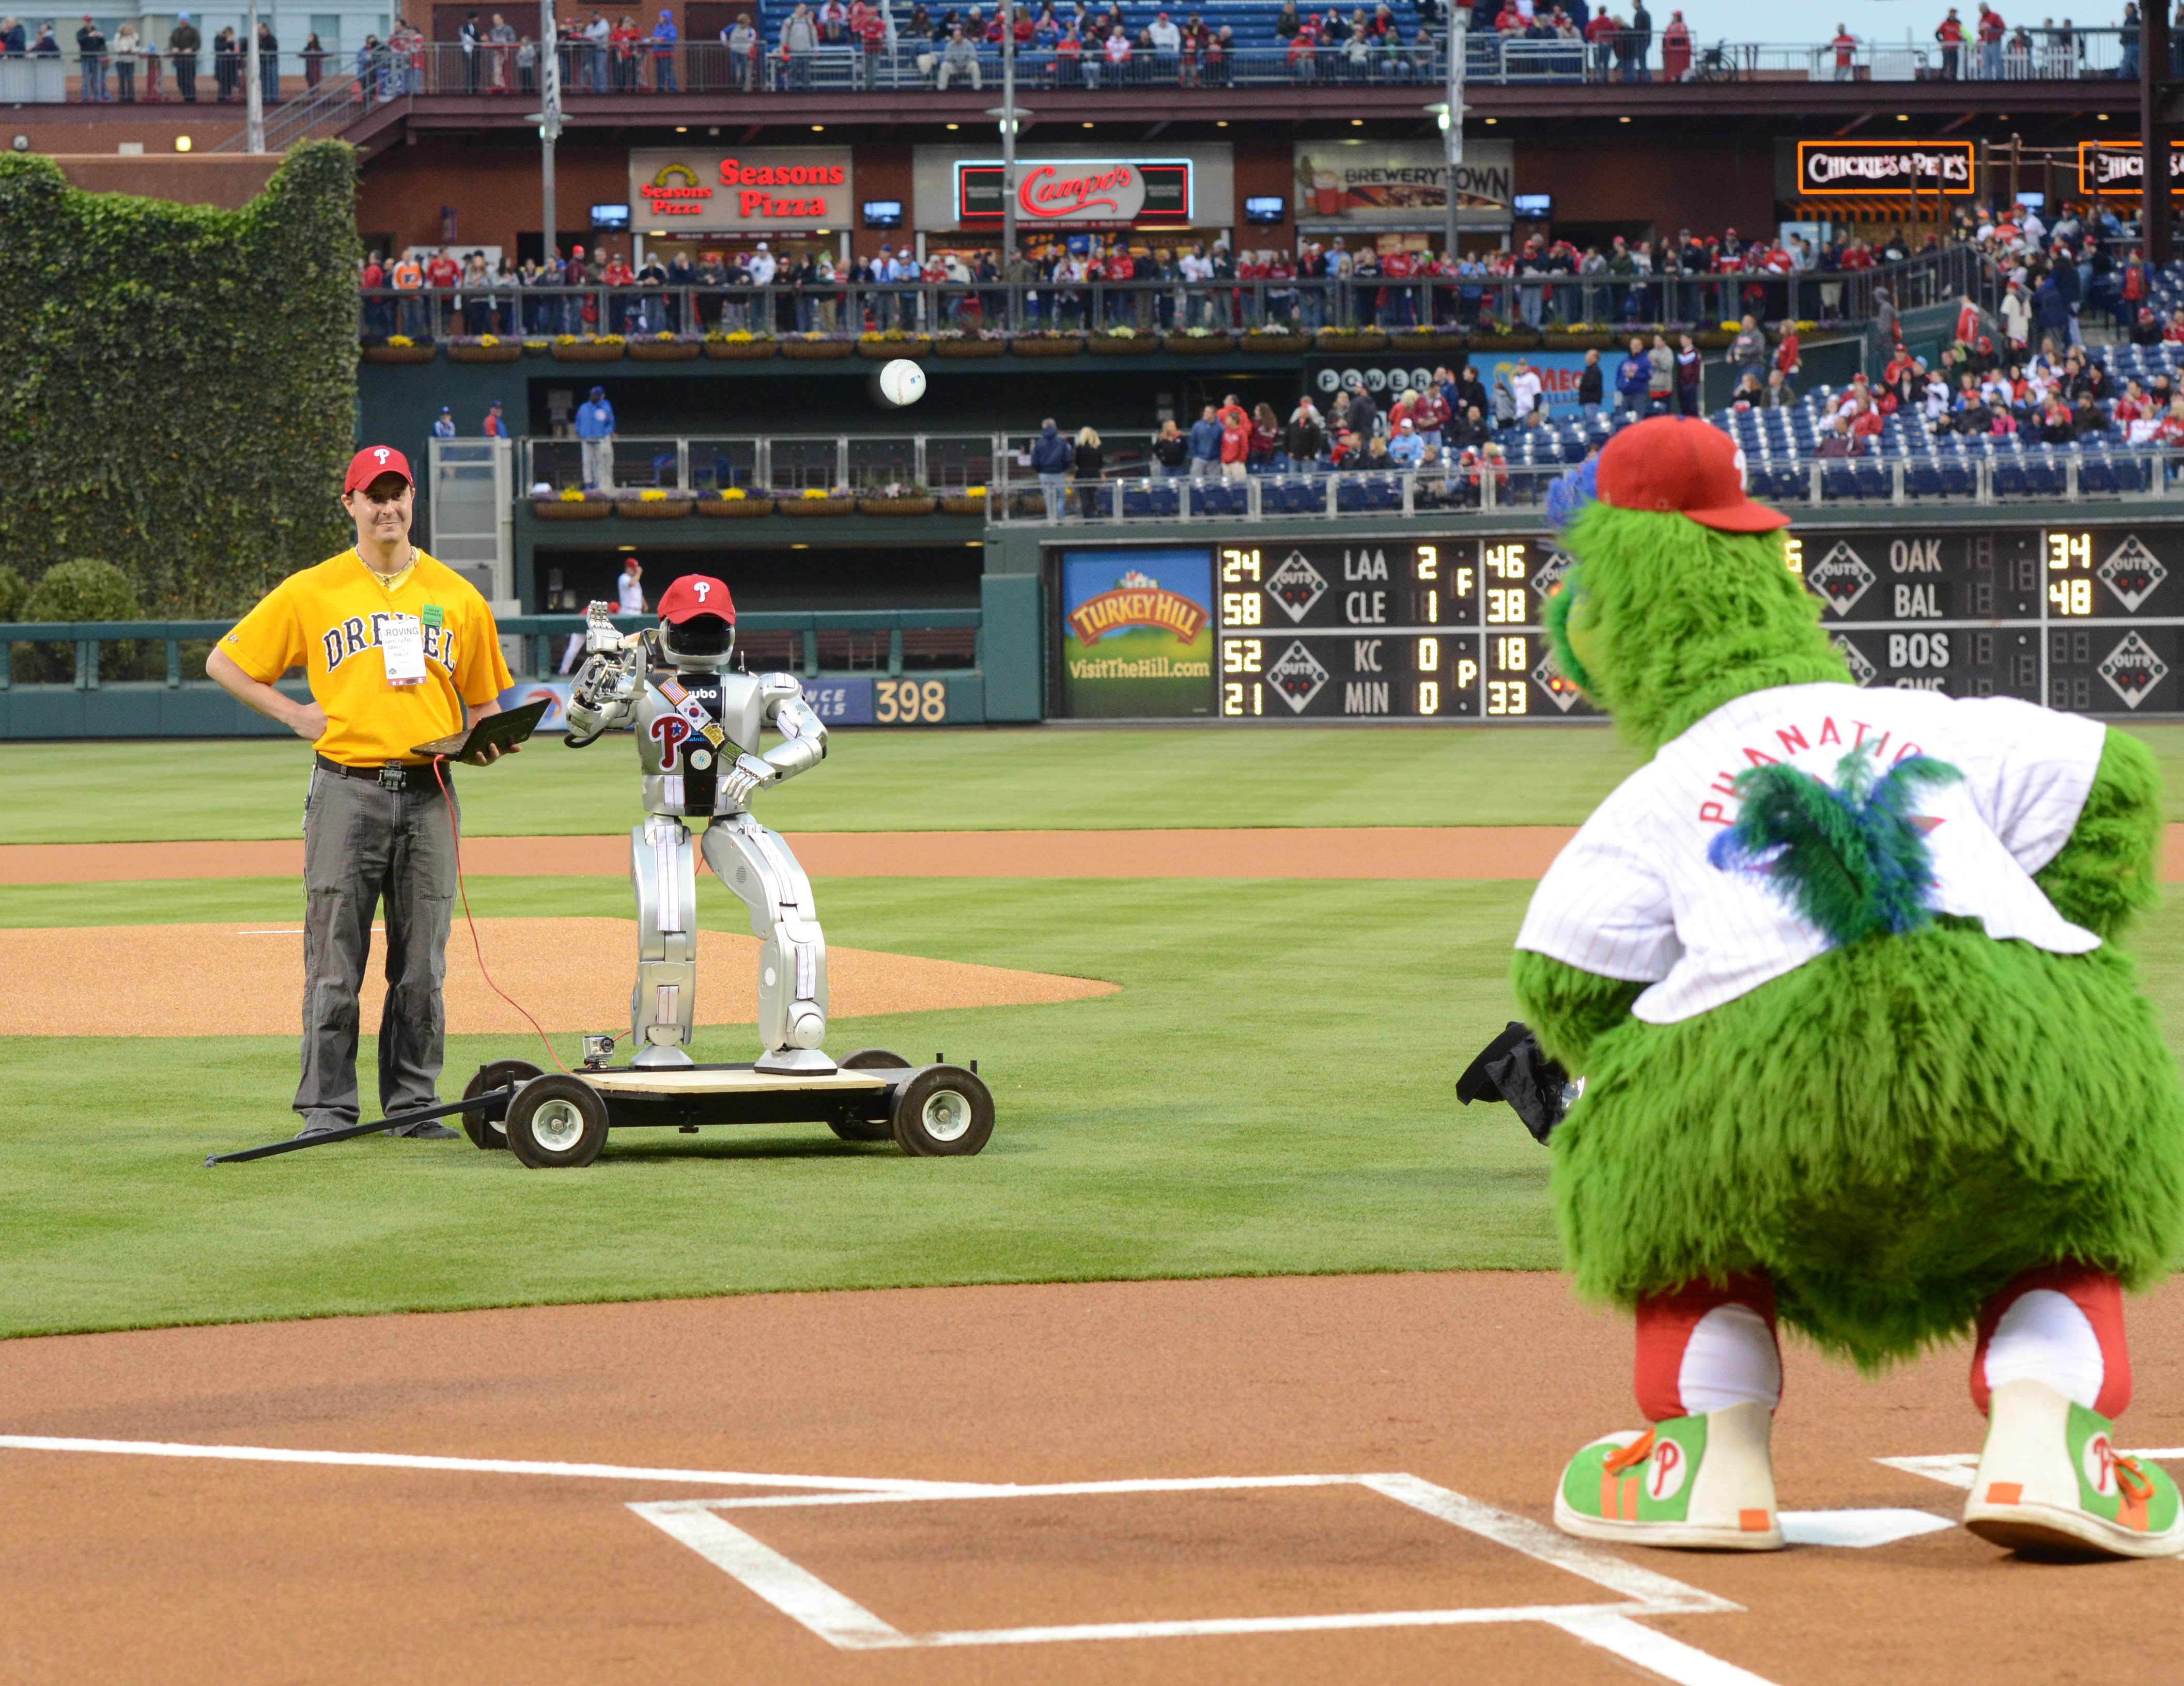
\includegraphics[width=1.0\columnwidth]{./pix/hubo-pitch.png}
  \caption{Hubo successfully throwing the first pitch at the second annual Philadelphia Science Festival event Science Night at the Ball Park on April 28th, 2012.  The game was between the Philadelphia Phillies and the Chicago Cubs and played at the Major League Baseball stadium Citizens Bank Park.  The Phillies won 5-2.  Video of the pitch can be found at http://danlofaro.com/urai2012/\#pitch}
  \label{fig:hubo-throw}
\end{figure}


%The PhillieBot\footnote{PhillieBot Video: http://youtu.be/ShId-vZ-ZEY} made by the GRASP Lab at the University of Pennsylvania was the robot that threw the first pitch at the first annual Philadelphia Science Festival \textit{Science Night at the Ballpark} in 2011.  

Hubo was the first full-size humanoid to throw the inaugural pitch at a Major League Baseball game.  
This task poses challenges in the area of fully-body locomotion, coordination and stabilization that must be addressed.
This paper describes how the latter was done via the analyses/tests of three different approaches and the resulting final design.
Section~\ref{sec:background} gives a brief introduction to work already done in the field as well as states the requirements for the pitch.
Section~\ref{sec:methodology} describes the three different methods tested with a focus on the human-robot kinematic mapping approach.  
The fully automated approach that uses the sparse reachable map (SRM)\cite{dlofaro-srm} and key-frame trajectory generation methods are also explored.
Section~\ref{sec:comparison} compares the tests and analyses of each of the methods.
Section~\ref{sec:finalDesign} describes the finial design in detail and the modifications needed to make the robot's pitch reliable.
Section~\ref{sec:conclusion} gives final thoughts and possible improvements for future years.


%% remember robust and to say that you learned from upenns mistakes etc.
\input{background.tex}
\input{methodology.tex}
\input{comparison.tex}
\input{finalDesign.tex}

\input{conclusion.tex}


% An example of a floating figure using the graphicx package.
% Note that \label must occur AFTER (or within) \caption.
% For figures, \caption should occur after the \includegraphics.
% Note that IEEEtran v1.7 and later has special internal code that
% is designed to preserve the operation of \label within \caption
% even when the captionsoff option is in effect. However, because
% of issues like this, it may be the safest practice to put all your
% \label just after \caption rather than within \caption{}.
%
% Reminder: the "draftcls" or "draftclsnofoot", not "draft", class
% option should be used if it is desired that the figures are to be
% displayed while in draft mode.
%
%\begin{figure}[!t]
%\centering
%\includegraphics[width=2.5in]{myfigure}
% where an .eps filename suffix will be assumed under latex, 
% and a .pdf suffix will be assumed for pdflatex; or what has been declared
% via \DeclareGraphicsExtensions.
%\caption{Simulation Results}
%\label{fig_sim}
%\end{figure}

% Note that IEEE typically puts floats only at the top, even when this
% results in a large percentage of a column being occupied by floats.


% An example of a double column floating figure using two subfigures.
% (The subfig.sty package must be loaded for this to work.)
% The subfigure \label commands are set within each subfloat command, the
% \label for the overall figure must come after \caption.
% \hfil must be used as a separator to get equal spacing.
% The subfigure.sty package works much the same way, except \subfigure is
% used instead of \subfloat.
%
%\begin{figure*}[!t]
%\centerline{\subfloat[Case I]\includegraphics[width=2.5in]{subfigcase1}%
%\label{fig_first_case}}
%\hfil
%\subfloat[Case II]{\includegraphics[width=2.5in]{subfigcase2}%
%\label{fig_second_case}}}
%\caption{Simulation results}
%\label{fig_sim}
%\end{figure*}
%
% Note that often IEEE papers with subfigures do not employ subfigure
% captions (using the optional argument to \subfloat), but instead will
% reference/describe all of them (a), (b), etc., within the main caption.


% An example of a floating table. Note that, for IEEE style tables, the 
% \caption command should come BEFORE the table. Table text will default to
% \footnotesize as IEEE normally uses this smaller font for tables.
% The \label must come after \caption as always.
%
%\begin{table}[!t]
%% increase table row spacing, adjust to taste
%\renewcommand{\arraystretch}{1.3}
% if using array.sty, it might be a good idea to tweak the value of
% \extrarowheight as needed to properly center the text within the cells
%\caption{An Example of a Table}
%\label{table_example}
%\centering
%% Some packages, such as MDW tools, offer better commands for making tables
%% than the plain LaTeX2e tabular whffich is used here.
%\begin{tabular}{|c||c|}
%\hline
%One & Two\\
%\hline
%Three & Four\\
%\hline
%\end{tabular}
%\end{table}


% Note that IEEE does not put floats in the very first column - or typically
% anywhere on the first page for that matter. Also, in-text middle ("here")
% positioning is not used. Most IEEE journals/conferences use top floats
% exclusively. Note that, LaTeX2e, unlike IEEE journals/conferences, places
% footnotes above bottom floats. This can be corrected via the \fnbelowfloat
% command of the stfloats package.







% conference papers do not normally have an appendix


% use section* for acknowledgement
\section*{Acknowledgment}

This project was conducted by the Drexel Autonomous Systems Lab (DASL), the Music Entertainment Technology Lab (MET)\footnote{Music Entertainment Technology Lab: http://music.ece.drexel.edu}, and sponsored by the National Science Foundation via the two grants; Partnerships for International Research and Education (\#0730206) and Major Research Infrastructure Recovery and Reinvestment (\#CNS-0960061).  Special thanks for organization and technical assistance goes to the Philadelphia Science Festival, Robert Ellenberg and Roy Gross.  The robot platform used was Hubo, designed and created by our partner Dr. Jun-Ho Oh, Department of Mechanical Engineering, Korean Advanced Institute of Science and Technology, Daejeon, South Korea.% <-this %





% trigger a \newpage just before the given reference
% number - used to balance the columns on the last page
% adjust value as needed - may need to be readjusted if
% the document is modified later
%\IEEEtriggeratref{8}
% The "triggered" command can be changed if desired:
%\IEEEtriggercmd{\enlargethispage{-5in}}

% references section

% can use a bibliography generated by BibTeX as a .bbl file
% BibTeX documentation can be easily obtained at:
% http://www.ctan.org/tex-archive/biblio/bibtex/contrib/doc/
% The IEEEtran BibTeX style support page is at:
% http://www.michaelshell.org/tex/ieeetran/bibtex/
%\bibliographystyle{IEEEtran}
% argument is your BibTeX string definitions and bibliography database(s)
%\bibliography{IEEEabrv,../bib/paper}
%
% <OR> manually copy in the resultant .bbl file
% set second argument of \begin to the number of references
% (used to reserve space for the reference number labels box)
%\begin{thebibliography}{1}

\bibliographystyle{IEEEtran}
%\bibliographystyle{plain}
\bibliography{throwing}{}
  
%\end{thebibliography}




% that's all folks
\end{document}


